	
	
	
	
	
	
	
	
	
	
	
	
	
	
	
	
	
	
	
	
	
	
	
	
	
	
	
	
	
	
	
	
	
	
	
	
	
	
	
	
	
	\section{Calcul des balcons}
	
	\subsection{Introduction}
	
	Le balcon est un espace extérieur ouvert, attaché à la façade d'un bâtiment, sans toit ni côtés fermés, à l'exception d'un garde-corps pour des raisons de sécurité.
	
	\vspace{\baselineskip}
	
	Les balcons seront généralement réalisés en dalles pleines encastrée dans des poutres
	horizontales, et peuvent être aussi réaliser en corps creux.
	
	Dans ce projet les balcons sont en \underline{dalle pleine de 15 cm d'épaisseur.}
	
	\subsection{Calcul des charges}
	
	Nous avons pour la surcharge d'exploitation : $Q_{balcon} = 3,5\knms$
	
	\vspace{\baselineskip}
	
	\begin{table}[H]
		\centering
		\caption{Descente des charges pour le balcon.}
		\label{tab:decente-charges-balcon}
		\begin{tabular}{|l|c|}
			\hline
			Types de charges & Valeur ($\knms$) \\ \hline
			Poids propres & $25 \times 0,15 = 3,75$ \\
			Couche de sable & 0,36 \\
			Mortier de pose & 0,4 \\
			Carrelage & 0,44 \\
			Poids des murs & 0,9 \\ \hline
			\multicolumn{1}{c|}{} & 5,85 \\ \cline{2-2}
			
		\end{tabular}
	\end{table}
	
	\begin{tcolorbox}[colback=gray!20, colframe=black, title=Remarque]
		Le poids du garde corps n'est pas prit en compte car on à ajouter le poids des murs qui est en $\msq$, donc on peut dire que le garde corps est inclus.
	\end{tcolorbox}
	
	\vspace{\baselineskip}
	
	Le calcul se fera pour 1ml donc la charge final est de : 
	
	\[ \fbox{$q = (1,35 \times 5,85 + 1,5 \times 3,5) \times 1ml = 13,14 \simeq 13 \knm$} \]
	
	
	\subsection{Schéma}
	
	Ce projet comporte deux balcons (types) : 
	
		
	\begin{multicols}{2}
		\begin{figure}[H]
			\centering
			\begin{tikzpicture}
				
				\draw[pattern=north west lines] (0,0) coordinate (a) rectangle (4,2.5) coordinate (b);
				
				\draw[fill=white] (.5,0) coordinate (c) rectangle (3.5,2) coordinate 	(d);
				
				
				\dimensioning{1}{a}{c}{-1}[20];
				\dimensioning{1}{c}{d}{-1}[190];
				\dimensioning{1}{d}{b}{-1}[20];
				
				\dimensioning{2}{a}{d}{-1}[140];
				\dimensioning{2}{d}{b}{-1}[20];
				
			\end{tikzpicture}
			\caption{Dimension d'un balcon (cas 1)}
			\label{fig:dim-balcon1}
		\end{figure}
		
		\columnbreak
		
		\begin{figure}[H]
			\centering
			\begin{tikzpicture}
				
				\draw[pattern=north west lines] (0,0) coordinate (a) rectangle (6,2.5) coordinate (b);
				
				\draw[fill=white] (.5,0) coordinate (c) rectangle (5.5,2) coordinate 	(d);
				
				\dimensioning{1}{a}{c}{-1}[20];
				\dimensioning{1}{c}{d}{-1}[270];
				\dimensioning{1}{d}{b}{-1}[20];
				
				\dimensioning{2}{d}{a}{7}[140];
				\dimensioning{2}{b}{d}{7}[20];
				
			\end{tikzpicture}
			\caption{Dimension d'un autre balcon (cas 2)}
			\label{fig:dim-balcon2}
		\end{figure}
	
	\end{multicols}
	
	{\centering Les hachures représente les poutres (l'encastrement du balcon.)\par}
	
	
	\subsection{Calcul des efforts internes}
	
	Avant de calculé les efforts internes, les sens porteur doivent être d'abord définie :
	
	Pour savoir le sens porteur on utilise cette formule :
	
	\[ \alpha = \dfrac{L_{x}}{L_{y}} \leq 0,4 \]
	
	Avec : $L_{y}$ la grande porté et $L_{x}$ la petite portée.
	
	Si la condition est vérifié donc la dalle pleine porte dans un seul sens sinon c'est dans les deux sens.
	
	\vspace{\baselineskip}
	
	\textbf{Cas 1}
	
	\[ \alpha = \dfrac{140}{190} = 0,73 > 0,4 \]
	
	{\centering Le panneau porte dans les deux sens\par}
	
	\textbf{Cas 2}
	
	\[ \alpha = \dfrac{140}{270} = 0,51 > 0,4 \]
	
	{\centering Le panneau porte dans les deux sens\par }
	
	
	\subsubsection{Calcul selon x--x}
	
	\begin{multicols}{2}
		
		\textbf{Premier cas}
		
		\begin{figure}[H]
			\centering
			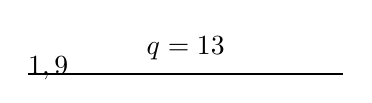
\begin{tikzpicture}
				
				\draw (0,0)coordinate (a) -- (4,0) coordinate (b) node[midway,above=1.5] {$q = 13\knm$};
				
				\support{3}{a}[-90];
				\support{3}{b}[90];
				
				\lineload{1}{a}{b}[1][1];
				
				\dimensioning{1}{a}{b}{-1}[$1,9\meterl$];
				
			\end{tikzpicture}
		\end{figure}
		
		
		
		\[ \fbox{$\begin{aligned}
				M_{A} = M_{B} = -\dfrac{q \times l^{2}}{12} &= -3,91\knxm \\
				M_{t_{A--B}} = \dfrac{q \times l^{2}}{24} &= 1,95\knxm \\
				V = \dfrac{ql}{2} &= 12,35\kn
			\end{aligned}$} \]
		
		
		
		
		\columnbreak
		
		
		
		
		
		
		
		
		
		\textbf{Deuxième cas}
		
		\begin{figure}[H]
			\centering
			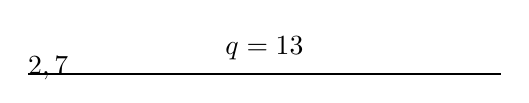
\begin{tikzpicture}
				
				\draw (0,0)coordinate (a) -- (6,0) coordinate (b) node[midway,above=1.5] {$q = 13\knm$};
				
				\support{3}{a}[-90];
				\support{3}{b}[90];
				
				\lineload{1}{a}{b}[1][1];
				
				\dimensioning{1}{a}{b}{-1}[$2,7\meterl$];
				
			\end{tikzpicture}
		\end{figure}
		
		
		\[ \fbox{$\begin{aligned}
				M_{A} = M_{B} = -\dfrac{q \times l^{2}}{12} &= -7,89\knxm \\
				M_{t_{A--B}} = \dfrac{q \times l^{2}}{24} &= 3,95\knxm \\
				V = \dfrac{ql}{2} &= 17,55\kn
			\end{aligned}$} \]
		
	\end{multicols}
	
	
	
	
	\subsubsection{Calcul selon y--y pour les deux cas}
	
	\begin{figure}[H]
		\centering
		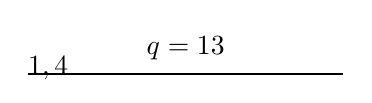
\begin{tikzpicture}
			
			\draw (0,0)coordinate (a) -- (4,0) coordinate (b) node[midway,above=1.5] {$q = 13\knm$};
			
			\support{3}{a}[-90];
			
			\lineload{1}{a}{b}[1][1];
			
			\dimensioning{1}{a}{b}{-1}[$1,4\meterl$];
			
		\end{tikzpicture}
	\end{figure}
	
	
	\[ \fbox{$\begin{aligned}
			M = -\dfrac{q \times l^{2}}{2} &= -12,74\knxm \\
			V = q \times l &= 18,2\kn 
		\end{aligned}$} \]
	
	
	
	
	\subsection{Calcul du ferraillage}
	
	\textbf{Données :} $\sgma{bc} = 14,2\mpa$, $\quad\sgma{st} = 348\mpa$, $\quad c = 3\cml \rightarrow d = 15 - 3 = 12\cml$
	
	
	\subsubsection{Mi-travée x--x}
	
	\begin{multicols}{2}
		
		\textbf{Cas 1}
		
		\[ \begin{aligned}
			\mu &= \dfrac{1,95}{100 \times 12^{2} \times 1,42} \\
			&= \num{9,53e-5} <<< \mu_{l} = 0,392
		\end{aligned} \]
		
		Vu la valeur très inférieur on peut dire que le béton suffit a reprendre ces efforts (section d'armature très petite).
		
		\columnbreak
		
		\textbf{Cas 2}
		
		\[ \begin{aligned}
			\mu &= \dfrac{3,95}{100 \times 12^{2} \times 1,42} \\
			&= \num{1,93e-4} <<< \mu_{l} = 0,392
		\end{aligned} \]
		
		\hspace{0.5cm} Même chose que dans le premier cas.
		
	\end{multicols}
	
	
	\subsubsection{En appui x--x}
	
	\textbf{Cas 1}
	
	Pour le premier cas en appuie on aura la même chose qu'on travée car les moment sont égaux (section d'armature très petite).
	
	\textbf{Cas 2}
	
	\[ \mu = \dfrac{7,9}{100 \times 12^{2} \times 1,42} = \num{3,86e-4} <<< \mu_{l} \]
	
	{\centering Pareil que les autres cas\par}
	
	\vspace{\baselineskip}
	
	\textbf{Condition non fragilité sur appuie et en travée}
	
	\[ \fbox{$A_{\min} = 0,23 \times \dfrac{0,21}{40} \times 100 \times 12 = 1,45\cmsq \rightarrow 5HA6 = 1,41\cmsq$} \]
	
	
	\subsubsection{En appui y--y}
	
	\[ \mu = \dfrac{12,74}{100 \times 12^{2} \times 1,42} = \num{6,23e-4} <<< \mu_{l} \]
	
	\[ \fbox{$A_{\min} = 1,45\cmsq \rightarrow 5HA6 = 1,41\cmsq$} \]
	
	\underline{\textbf{Avec un espacement de $15\cml$}}
	
	
	\subsection{Plan de ferraillage}
	
	
	
	\begin{figure}[H]
		\centering
		\includegraphics[width=0.7\linewidth]{"../figures/Chapitre 3/ferraillage-balcon"}
		\caption{Plan de ferraillage du balcon}
		\label{fig:ferraillage-balcon}
	\end{figure}
	
	
	
	
	
	
	
	
	
	
